\documentclass{article}

\usepackage{epsfig}  
\usepackage{amsmath} 
\usepackage{amssymb} 
\usepackage{amsthm}  
\usepackage{listings} 
\usepackage{color}
%\usepackage{enumerate}
\usepackage{enumitem}
\usepackage{multirow}
\usepackage{lastpage}
\usepackage{geometry}
\usepackage{fancyhdr}
\usepackage[all]{xy}
\usepackage{wrapfig}
\usepackage{listings}
\usepackage{url}
\usepackage{tikz}
\usepackage{graphicx}
\usepackage{caption}
\usepackage{subcaption}
\usepackage[justification=centering]{caption}
\usetikzlibrary{arrows}
\lstset{language=C, tabsize=4, basicstyle=\ttfamily}

\definecolor{light}{gray}{.75} 
\newtheorem{theorem}{Theorem}



\pagestyle{fancy}
\lhead{CSCE 990 - FALL 2014} 
\chead{\bfseries PROJECT PROPOSAL}
\rhead{Gerrard, Ore}
\lfoot{Gerrard, Ore}
\cfoot{\thepage\ of \pageref{LastPage}}
\rfoot{3 November 2014}
\renewcommand{\headrulewidth}{0.4pt}
\renewcommand{\footrulewidth}{0.4pt}

\hoffset 0pt
\voffset 0pt
\textwidth 15cm
\textheight 8.5in
\oddsidemargin 9pt
\marginparwidth 25pt
\setlength{\parindent}{0pt}
\setlength{\parskip}{.25cm}

%- - - - - - - - - - - - - - - - BEGIN DOCUMENT - - - - - - - - - - - - - - - - - - - 
\begin{document}


\section{Target Problem Description}
\cite{schneider2010synoptic}



Model extraction seeks to help developers understand complex systems by finding a simplified representation that still retains useful high-level information.
This high-level information helps validate assumptions about the system's behavior or to discover counter-examples that violate implicit requirements of a system's behavior.
The system's behavior is often recorded in system logs or execution traces, that provide some facts about the behavior of the system but are sometimes overwhelmingly massive and difficult to connect to high-level facts, even though these facts might reveal critical information about the behavior of the system.

One tool that helps extract model from computer execution traces is Synoptic, that takes system event logs as input and extracts high-level models based on calculating invariants and coarsening and refining an abstract model.
Synoptic and other tools usually work at an abstract level of system events, that happen in a particular order.
We are interested in applying event model extraction techniques in the robotic domain, wherein events happen in both \emph{time} and \emph{spatial} domains.

The problem is to explore if model extraction techniques that are usually applied to temporal events (like network program execution traces) can be applied to spatial robotic data.

There are several challenges in this endeavor, including mapping existing robotic system trace data to \emph{events}, so that the spatial relationships of these events can be explored by extending previous model extraction techniques. 

\section{Sketch of technique}

We start with robotic system traces from ROS, a published-subscriber architecture for connecting robotic components.  
These traces are called `bags' within the domain of ROS, and contain system messages published on certain data structures (called topics) in chronological order.
Specifically, we will examine trace data from a UAV system used to collect water samples during windy conditions.
Each file might contain 100,000 records, and we have 50-100 bags.

Starting with these bags, we plan to create functions that recognize certain sequences and values of message and record `events' to a new event log.
This event log captures important spatial events during the execution of an automated script, or plan, that lasts about five minutes.
One of the challenges will be creating the functions that recognize these events and determining the correct level of refinement for these events.



%\begin{figure}[b]
    %\centering
    %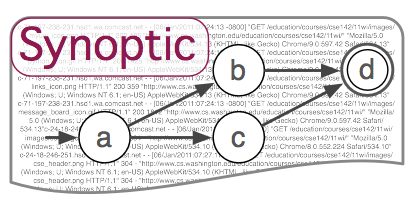
\includegraphics[width=0.4\textwidth]{./figures/TBD.jpg}
    %\caption{Awesome Image}
    %\label{fig:awesome_image}
%\end{figure}


\section{Expected Outcome} 


\bibliographystyle{IEEEtran}
\bibliography{IEEEabrv,refs.bib}

\end{document}
